\chapter{Vector spaces}
\label{ch:vector_spaces}
This is a pretty light chapter.
The point of it is to define what a vector space and a basis are.
These are intuitive concepts that you may already know.

\section{The definitions of a ring and field}
\prototype{$\ZZ$, $\RR$, and $\CC$ are rings; the latter two are fields.}

I'll very informally define a ring/field here,
in case you skipped the earlier chapter.
\begin{itemize}
	\ii A \textbf{ring} is a structure with a \emph{commutative}
	addition and multiplication, as well as subtraction, like $\ZZ$.
	It also has an additive identity $0$ and multiplicative identity $1$.

	\ii If the multiplication is invertible like in $\RR$ or $\CC$,
	(meaning $\frac 1x$ makes sense for any $x \neq 0$),
	then the ring is called a \textbf{field}.
\end{itemize}
In fact, if you replace ``field'' by ``$\RR$'' everywhere in what follows,
you probably won't lose much.
It's customary to use the letter $R$ for rings, and $k$ or $K$ for fields.

Finally, in case you skipped the chapter on groups, I should also mention:
\begin{itemize}
	\ii An \textbf{additive abelian group} is a structure
	with a commutative addition, as well as subtraction,
	plus an additive identity $0$.
	It doesn't have to have multiplication.
	A good example is $\RR^3$ (with addition componentwise).
\end{itemize}

\section{Modules and vector spaces}
\prototype{Polynomials of degree at most $n$.}
You intuitively know already that $\RR^n$ is a ``vector space'':
its elements can be added together,
and there's some scaling by real numbers.
Let's develop this more generally.

Fix a commutative ring $R$.
Then informally,
\begin{moral}
	An $R$-module is any structure where you can add two elements
	and scale by elements of $R$.
\end{moral}
% You can think of the $R$-module as consisting of soldiers
% being commanded by the ring $R$.
Moreover, a \vocab{vector space} is just a module whose commutative ring
is actually a field.
I'll give you the full definition in a moment,
but first, examples\dots

\begin{example}
	[Quadratic polynomials, aka my favorite example]
	My favorite example of an $\RR$-vector space is the
	set of polynomials of degree at most two, namely
	\[ \left\{ ax^2+bx+c \mid a,b,c \in \RR \right\}. \]
	Indeed, you can add any two quadratics, and multiply by constants.
	You can't multiply two quadratics to get a quadratic,
	but that's irrelevant -- in a vector space there need not
	be a notion of multiplying two vectors together.

	In a sense we'll define later, this vector space
	has dimension $3$ (as expected!).
	% But I hope you can see why this is kind of true!
	\label{ex:quadratic_vector_space}
\end{example}
\begin{example}[All polynomials]
	The set of \emph{all} polynomials with real coefficients is an
	$\RR$-vector space, because you can \emph{add any two polynomials}
	and \emph{scale by constants}.
\end{example}

\begin{example}
	[Euclidean space]
	\listhack
	\begin{enumerate}[(a)]
		\ii The complex numbers
		\[ \left\{ a+bi \mid a,b \in \RR \right\} \]
		form a real vector space. As we'll see later,
		it has ``dimension $2$''.
		\ii The real numbers $\RR$ form a real vector space of dimension $1$.
		\ii The set of 3D vectors
		\[ \left\{ (x,y,z) \mid x,y,z \in \RR \right\} \]
		forms a real vector space, because you can add any two triples
		component-wise. Again, we'll later explain
		why it has ``dimension $3$''.
	\end{enumerate}
\end{example}

\begin{example}
	[More examples of vector spaces]
	\listhack
	\begin{enumerate}[(a)]
		\ii The set \[ \QQ[\sqrt 2] = \left\{ a + b \sqrt 2 \mid a, b \in \QQ \right\} \]
		has a structure of a $\QQ$-vector space in the obvious fashion:
		one can add any two elements, and scale by rational numbers.
		(It is not an $\RR$-vector space --- why?)
		\ii The set \[ \left\{ (x,y,z) \mid x+y+z = 0 \text{ and } x,y,z \in \RR \right\} \]
		is a $2$-dimensional real vector space.
		\ii The set of all functions $f \colon \RR \to \RR$ is also a real vector space
		(since the notions $f+g$ and $c \cdot f$ both make sense for $c \in \RR$).
	\end{enumerate}
\end{example}

Now let me write the actual rules for how this multiplication behaves.
\begin{definition}
	Let $R$ be a commutative ring.
	An $R$-\vocab{module} starts with an additive abelian group $M = (M,+)$
	whose identity is denoted $0 = 0_M$.
	We additionally specify a left multiplication by elements of $R$.
	This multiplication must satisfy the following properties
	for $r, r_1, r_2 \in R$ and $m, m_1, m_2 \in M$:
	\begin{enumerate}[(i)]
		\ii $r_1 \cdot (r_2 \cdot m) = (r_1r_2) \cdot m$.
		\ii Multiplication is distributive, meaning
		\[ (r_1+r_2) \cdot m = r_1 \cdot m + r_2 \cdot m
			\text{ and }
			r \cdot (m_1 + m_2) = r \cdot m_1 + r \cdot m_2. \]
		\ii $1_R \cdot m = m$.
		\ii $0_R \cdot m = 0_M$.
		(This is actually extraneous;
		one can deduce it from the first three.)
	\end{enumerate}
	If $R$ is a field we say $M$ is an $R$-\vocab{vector space};
	its elements are called \vocab{vectors}
	and the members of $R$ are called \vocab{scalars}.
\end{definition}

\begin{abuse}
	In the above, we're using the same symbol $+$ for the addition of $M$
	and the addition of $R$.
	Sorry about that, but it's kind of hard to avoid, and the point
	of the axioms is that these additions should be related.
	I'll try to remember to put $r \cdot m$ for the multiplication of the module
	and $r_1r_2$ for the multiplication of $R$.
\end{abuse}

\begin{ques}
	In \Cref{ex:quadratic_vector_space},
	I was careful to say ``degree at most $2$'' instead of ``degree $2$''.
	What's the reason for this?
	In other words, why is
	\[ \left\{ ax^2 + bx + c \mid a,b,c \in \RR, a \neq 0  \right\} \]
	not an $\RR$-vector space?
\end{ques}

A couple less intuitive but somewhat important examples\dots
\begin{example}[Abelian groups are $\ZZ$-modules]
	(Skip this example if you're not comfortable with groups.)
	\begin{enumerate}[(a)]
		\ii The example of real polynomials
		\[ \left\{ ax^2+bx+c \mid a,b,c \in \RR \right\} \]
		is also a $\ZZ$-module!
		Indeed, we can add any two such polynomials,
		and we can scale them by integers.
		\ii The set of integers modulo $100$, say $\ZZ/100\ZZ$,
		is a $\ZZ$-module as well. Can you see how?
		\ii In fact, \emph{any} abelian group $G = (G,+)$ is a $\ZZ$-module.
		The multiplication can be defined by
		\[ n \cdot g = \underbrace{g+\dots+g}_{\text{$n$ times}}
		\qquad (-n) \cdot g = n \cdot (-g)\]
		for $n \ge 0$. (Here $-g$ is the additive inverse of $g$.)
	\end{enumerate}
\end{example}
\begin{example}
	[Every ring is its own module]
	\listhack
	\begin{enumerate}[(a)]
	\ii $\RR$ can be thought of as an $\RR$-vector space over itself.
	Can you see why?

	\ii By the same reasoning,
	we see that \emph{any} commutative ring $R$ can be thought of
	as an $R$-module over itself.
	\end{enumerate}
\end{example}

\section{Direct sums}
\prototype{$\{ax^2+bx+c\} = \RR \oplus x\RR \oplus x^2\RR$, and
$\RR^3$ is the sum of its axes.}
Let's return to \Cref{ex:quadratic_vector_space}, and consider
\[ V = \left\{ ax^2+bx+c \mid a,b,c \in \RR \right\}.  \]
Even though I haven't told you what a dimension is,
you can probably see that this vector space ``should have'' dimension $3$.
We'll get to that in a moment.

The other thing you may have noticed is that somehow
the $x^2$, $x$ and $1$ terms don't ``talk to each other''.
They're totally unrelated.
In other words, we can consider the three sets
\begin{align*}
	x^2\RR &\defeq \left\{ ax^2 \mid a \in \RR \right\} \\
	x\RR &\defeq \left\{ bx \mid b \in \RR \right\} \\
	\RR &\defeq \left\{ c \mid c \in \RR \right\}.
\end{align*}
In an obvious way, each of these can be thought of as a ``copy'' of $\RR$.

Then $V$ quite literally consists of the ``sums of these sets''.
Specifically, every element of $V$ can be written \emph{uniquely}
as the sum of one element from each of these sets.
This motivates us to write
\[ V = x^2\RR \oplus x\RR \oplus \RR. \]
The notion which captures this formally is the \vocab{direct sum}.

\begin{definition}
	\label{def:vector_space_direct_sum}
	Let $M$ be an $R$-module.
	Let $M_1$ and $M_2$ be subsets of $M$ which are themselves $R$-modules.
	Then we write $M = M_1 \oplus M_2$ and say $M$ is a \vocab{direct sum}
	of $M_1$ and $M_2$
	if every element from $M$ can be written uniquely as the sum
	of an element from $M_1$ and $M_2$.
\end{definition}
\begin{example}[Euclidean plane]
	Take the vector space $\RR^2 = \left\{ (x,y) \mid x \in \RR, y \in \RR \right\}$.
	We can consider it as a direct sum of its $x$-axis and $y$-axis:
	\[ X = \left\{ (x,0) \mid x \in \RR  \right\}
		\text{ and }
		Y = \left\{ (0,y) \mid y \in \RR \right\}. \]
	Then $\RR^2 = X \oplus Y$.
\end{example}

This gives us a ``top-down'' way to break down modules
into some disconnected components.

By applying this idea in reverse, we can also construct
new vector spaces as follows.
In a very unfortunate accident, the two names and notations for technically
distinct things are exactly the same.
\begin{definition}
	Let $M$ and $N$ be $R$-modules.
	We define the \vocab{direct sum} $M \oplus N$
	to be the $R$-module whose elements are pairs $(m,n) \in M \times N$.
	The operations are given by
	\[ (m_1, n_1) + (m_2, n_2) = (m_1+m_2, n_1+n_2). \]
	and
	\[ r \cdot (m, n) = (r \cdot m, r \cdot n). \]
\end{definition}

For example, while we technically wrote $\RR^2 = X \oplus Y$,
since each of $X$ and $Y$ is a copy of $\RR$,
we might as well have written $\RR^2 \cong \RR \oplus \RR$.

\begin{abuse}
	The above illustrates an abuse of notation in the way we write a direct sum. The symbol $\oplus$ has two meanings.
	\begin{itemize}
		\ii If $V$ is a \emph{given} space and $W_1$ and $W_2$ are subspaces, then $V = W_1 \oplus W_2$ means that ``$V$ \emph{splits} as a direct sum $W_1 \oplus W_2$'' in the way we defined above.
		\ii If $W_1$ and $W_2$ are two \emph{unrelated} spaces, then $W_1 \oplus W_2$ is \emph{defined} as the vector space whose \emph{elements} are pairs $(w_1, w_2) \in W_1 \times W_2$.
	\end{itemize}
	You can see that these definitions ``kind of'' coincide.
\end{abuse}

In this way, you can see that $V$ should be isomorphic
to $\RR \oplus \RR \oplus \RR$;
we had $V = x^2\RR \oplus x\RR \oplus \RR$,
but the $1$, $x$, $x^2$ don't really talk to each other
and each of the summands is really just a copy of $\RR$ at heart.

\begin{definition}
	We can also define, for every positive integer $n$, the module
	\[ M^{\oplus n}
		\defeq \underbrace{M \oplus M \oplus \dots \oplus M}_{\text{$n$ times}}. \]
\end{definition}

\section{Linear independence, spans, and basis}
\prototype{%
	$\left\{ 1,x,x^2 \right\}$ is a basis of
	$\left\{ ax^2 + bx + c \mid a,b,c \in \RR \right\}$.}

The idea of a basis, the topic of this section,
gives us another way to capture the notion that
\[ V = \left\{ ax^2+bx+c \mid a,b,c \in \RR \right\} \]
is sums of copies of $\{1,x,x^2\}$.
This section should be very intuitive, if technical.
If you can't see why the theorems here ``should'' be true,
you're doing it wrong.

Let $M$ be an $R$-module now.
We define three very classical notions that you likely are already familiar with.
If not, fall upon your notion of Euclidean space or $V$ above.
\begin{definition}
	A \vocab{linear combination} of some vectors $v_1, \dots, v_n$
	is a sum of the form $r_1 v_1 + \dots + r_n v_n$,
	where $r_1, \dots, r_n \in R$.
	The linear combination is called \vocab{trivial}
	if $r_1 = r_2 = \dots = r_n = 0_R$, and \vocab{nontrivial} otherwise.
\end{definition}
\begin{definition}
	Consider a finite set of vectors $v_1, \dots, v_n$ in a module $M$.
	\begin{itemize}
		\ii It is called \vocab{linearly independent} if there
		is no nontrivial linear combination with value $0_M$.
		(Observe that $0_M = 0 \cdot v_1 + 0 \cdot v_2 + \dots + 0 \cdot v_n$
		is always true -- the assertion is that there is no other
		way to express $0_M$ in this form.)
		\ii It is called a \vocab{generating set} if every $v \in M$ can be written as
		a linear combination of the $\{v_i\}$.
		If $M$ is a vector space we say it is \vocab{spanning} instead.
		\ii It is called a \vocab{basis} (plural \vocab{bases})
		if every $v \in M$ can be written
		\emph{uniquely} as a linear combination of the $\{v_i\}$.
	\end{itemize}
	The same definitions apply for an infinite set, with the proviso
	that all sums must be finite.

\end{definition}
So by definition, $\left\{ 1,x,x^2 \right\}$ is a basis for $V$.
It's not the only one: $\{2, x, x^2\}$ and $\{x+4, x-2, x^2+x\}$
are other examples of bases, though not as natural.
However, the set $S = \{3+x^2, x+1, 5+2x+x^2\}$ is not a basis;
it fails for two reasons:
\begin{itemize}
	\ii Note that
	$0 = (3+x^2) + 2(x+1) - (5+2x+x^2)$.
	So the set $S$ is not linearly independent.
	\ii It's not possible to write $x^2$ as a sum of elements of $S$.
	So $S$ fails to be spanning.
\end{itemize}
With these new terms, we can say a basis is a linearly independent and spanning set.

\begin{example}[More examples of bases]
	\listhack
	\begin{enumerate}[(a)]
		\ii Regard $\QQ[\sqrt2]
		= \left\{ a + b \sqrt 2 \mid a, b \in \QQ \right\}$
		as a $\QQ$-vector space.
		Then $\{1, \sqrt 2\}$ is a basis.
		\ii If $V$ is the set of all real polynomials,
		there is an infinite basis $\{1, x, x^2, \dots\}$.
		The condition that we only use finitely many terms just says
		that the polynomials must have finite degree (which is good).
		\ii Let $V = \{ (x,y,z) \mid x+y+z=0 \text{ and } x,y,z \in \RR\}$.
		Then we expect there to be a basis of size $2$, but unlike previous examples
		there is no immediately ``obvious'' choice.
		Some working examples include:
		\begin{itemize}
			\ii $(1,-1,0)$ and $(1,0,-1)$,
			\ii $(0,1,-1)$ and $(1,0,-1)$,
			\ii $(5,3,-8)$ and $(2,-1,-1)$.
		\end{itemize}
	\end{enumerate}
\end{example}

\begin{exercise}
	Show that a set of vectors is a basis if and only if
	it is linearly independent and spanning.
	(Think about the polynomial example if you get stuck.)
\end{exercise}

Now we state a few results which assert
that bases in vector spaces behave as nicely as possible.
\begin{theorem}[Maximality and minimality of bases]
	\label{thm:vector_best}
	Let $V$ be a vector space over some field $k$
	and take $e_1, \dots, e_n \in V$. The following are equivalent:
	\begin{enumerate}[(a)]
		\ii The $e_i$ form a basis.
		\ii The $e_i$ are spanning, but no proper subset is spanning.
		\ii The $e_i$ are linearly independent, but adding any other
		element of $V$ makes them not linearly independent.
	\end{enumerate}
\end{theorem}
\begin{remark}
	If we replace $V$ by a general module $M$ over a commutative ring $R$,
	then (a) $\implies$ (b) and (a) $\implies$ (c) but not conversely.
\end{remark}
\begin{proof}
	Straightforward, do it yourself if you like.
	The key point to notice is that you need to divide by scalars for the converse direction,
	hence $V$ is required to be a vector space instead of just a module
	for the implications (b) $\implies$ (a) and (c) $\implies$ (a).
\end{proof}

\begin{theorem}
	[Dimension theorem for vector spaces]
	\label{thm:dimension_theorem}
	If a vector space $V$ has a finite basis,
	then every other basis has the same number of elements.
\end{theorem}
\begin{proof}
	We prove something stronger:
	Assume $v_1, \dots, v_n$ is a spanning set
	while $w_1, \dots, w_m$ is linearly independent. We claim that $n \ge m$.
	\begin{ques}
		Show that this claim is enough to imply the theorem.
	\end{ques}

	Let $A_0 = \{v_1, \dots, v_n\}$ be the spanning set.
	Throw in $w_1$: by the spanning condition,
	$w_1 = c_1 v_1 + \dots + c_n v_n$.
	There's some nonzero coefficient, say $c_n$.
	Thus \[ v_n = \frac{1}{c_n} w_1 - \frac{c_1}{c_n}v_1 - \frac{c_2}{c_n}v_2 - \dots. \]
	Thus $A_1 = \{v_1, \dots, v_{n-1}, w_1\}$ is spanning.
	Now do the same thing, throwing in $w_2$,
	and deleting some element of the $v_i$ as before to get $A_2$;
	the condition that the $w_i$ are linearly independent
	ensures that some $v_i$ coefficient
	must always not be zero.
	Since we can eventually get to $A_m$, we have $n \ge m$.
\end{proof}
\begin{remark*}
	[Generalizations]
	\hfill
	\begin{itemize}
		\ii The theorem is true for an infinite basis as well
		if we interpret ``the number of elements'' as ``cardinality''.
		This is confusing on a first read through, so we won't elaborate.
		\ii In fact, this is true for modules over any commutative ring.
		Interestingly, the proof for the general case proceeds by reducing
		to the case of a vector space.
	\end{itemize}
\end{remark*}

The dimension theorem, true to its name,
lets us define the \vocab{dimension} of
a vector space as the size of any finite basis, if one exists.
When it does exist we say $V$ is \vocab{finite-dimensional}.
So for example,
\[ V = \left\{ ax^2 + bx + c \mid a,b,c \in \RR \right\} \]
has dimension three, because $\left\{ 1,x,x^2 \right\}$ is a basis.
That's not the only basis: we could as well have written
\[ \left\{ a(x^2-4x) + b(x+2) + c \mid a,b,c \in \RR \right\} \]
and gotten the exact same vector space.
But the beauty of the theorem is that no matter how we try
to contrive the generating set, we always will get exactly three elements.
That's why it makes sense to say $V$ has dimension three.

On the other hand, the set of all polynomials
$\RR[x]$ is \emph{infinite-dimensional}
(which should be intuitively clear).

A basis $e_1, \dots, e_n$ of $V$ is really cool
because it means that to specify $v \in V$,
I only have to specify $a_1, \dots, a_n \in k$,
and then let $v = a_1 e_1 + \dots + a_n e_n$.
You can even think of $v$ as $\left( a_1, \dots, a_n \right)$.
% In a way I'll make precise in a moment, $V$ is actually isomorphic to just $k^{\oplus n}$.
To put it another way, if $V$ is a $k$-vector space we always have
\[ V = e_1 k \oplus e_2 k \oplus \dots \oplus e_n k. \]

\section{Linear maps}
\label{sec:vector_space_linear_maps}
\prototype{Evaluation of $\{ax^2+bx+c\}$ at $x=3$.}
We've seen homomorphisms and continuous maps.
Now we're about to see linear maps, the structure preserving maps
between vector spaces. Can you guess the definition?

\begin{definition}
	Let $V$ and $W$ be vector spaces over the same field $k$.
	A \vocab{linear map} is a map $T \colon V \to W$ such that:
	\begin{enumerate}[(i)]
		\ii We have $T(v_1 + v_2) = T(v_1) + T(v_2)$
		for any $v_1, v_2 \in V$.\footnote{In group language,
			$T$ is a homomorphism $(V,+) \to (W,+)$.}
		\ii For any $a \in k$ and $v \in V$, $T(a \cdot v) = a \cdot T(v)$.
	\end{enumerate}
	If this map is a bijection (equivalently, if it has an inverse),
	it is an \vocab{isomorphism}.
	We then say $V$ and $W$ are \vocab{isomorphic}
	vector spaces and write $V \cong W$.
\end{definition}

\begin{example}[Examples of linear maps]
	\listhack
	\begin{enumerate}[(a)]
		\ii For any vector spaces $V$ and $W$ there is a trivial linear map sending everything to $0_W \in W$.
		\ii For any vector space $V$, there is the identity isomorphism $\id \colon V \to V$.
		\ii The map $\RR^3 \to \RR$ by $(a,b,c) \mapsto 4a+2b+c$ is a linear map.
		\ii Let $V$ be the set of real polynomials of degree at most $2$.
		The map $\RR^3 \to V$ by $(a,b,c) \mapsto ax^2+bx+c$ is an \emph{isomorphism}.
		\ii Let $V$ be the set of real polynomials of degree at most $2$.
		The map $V \to \RR$ by $ax^2+bx+c \mapsto 9a + 3b + c$
		is a linear map, which can be described as ``evaluation at $3$''.
		\ii Let $W$ be the set of functions $\RR \to \RR$.
		The evaluation map $W \to \RR$ by $f \mapsto f(0)$ is a linear map.
		\ii There is a map of $\QQ$-vector spaces $\QQ[\sqrt2] \to \QQ[\sqrt2]$
		called ``multiply by $\sqrt2$''; this map sends $a+b\sqrt2 \mapsto 2b + a\sqrt2$.
		This map is an isomorphism, because it has an inverse ``multiply by $1/\sqrt2$''.
	\end{enumerate}
\end{example}

In the expression $T(a \cdot v) = a \cdot T(v)$, note that the first $\cdot$ is the multiplication of $V$ and the second $\cdot$ is the multiplication of $W$.
Note that this notion of isomorphism really only cares about the size of the basis:
\begin{proposition}[$n$-dimensional vector spaces are isomorphic]
	If $V$ is an $n$-dimensional vector space, then
	$V \cong k^{\oplus n}$.
\end{proposition}
\begin{ques}
	Let $e_1$, \dots, $e_n$ be a basis for $V$.
	What is the isomorphism?
	(Your first guess is probably right.)
\end{ques}
\begin{remark}
	You could technically say that all finite-dimensional vector
	spaces are just $k^{\oplus n}$ and that no other space is worth
	caring about.
	But this seems kind of rude.
	Spaces often are more than just triples: $ax^2+bx+c$ is a polynomial,
	and so it has some ``essence'' to it that you'd lose if you
	compressed it into $(a,b,c)$.

	Moreover, a lot of spaces, like the set of vectors $(x,y,z)$ with $x+y+z=0$,
	do not have an obvious choice of basis.
	Thus to cast such a space into $k^{\oplus n}$
	would require you to make arbitrary decisions.
\label{rem:vector_spaces_have_essence}
\end{remark}

\section{What is a matrix?}
Now I get to tell you what a matrix is!
This is fun, because now I can finally explain to you how to \emph{derive}
the recipes for matrix multiplication, rather than being told.

This section is so important, and also revelatory for so many students,
that I'm actually going to do it twice.
The first time, I'm going to work in an extremely special case,
namely $V = W = \RR^2$, using lots of numbers.
(This is how I explained this concept when I taught it to first-year
undergraduate students that didn't have proof experience.)
Then the second time, we'll do it in modern language without all the numbers.

\subsection{Extended example with $\RR^2$, suitable for the general public}
Throughout this section, I'll work specifically with $\RR^2$, whose elements
I will write as $\left[ \begin{smallmatrix} x \\ y \end{smallmatrix} \right]$ rather than $(x,y)$
(you'll see why when I talk about matrix multiplication).

Pop quiz:
\begin{itemize}
	\ii \textbf{Question 1}:
	Suppose that you're given a linear map $T \colon \RR^2 \to \RR^2$ such that
	$T\left( \left[ \begin{smallmatrix} 3 \\ 4 \end{smallmatrix} \right] \right)
	= \left[ \begin{smallmatrix} \pi \\ 9 \end{smallmatrix} \right]$
	and
	$T\left( \left[ \begin{smallmatrix} 100 \\ 100 \end{smallmatrix} \right] \right)
	= \left[ \begin{smallmatrix} 0 \\ 12 \end{smallmatrix} \right]$.
	What are
	$T\left( \left[ \begin{smallmatrix} 103 \\ 104 \end{smallmatrix} \right] \right)$ and
	$T\left( \left[ \begin{smallmatrix} 203 \\ 204 \end{smallmatrix} \right] \right)$?

	\textbf{Answer 1}: just add them.
	\begin{align*}
		T\left( \begin{bmatrix} 103 \\ 104  \end{bmatrix} \right)
		&= \begin{bmatrix} \pi \\ 9 \end{bmatrix}
		+ \begin{bmatrix} 0 \\ 12 \end{bmatrix}
		= \begin{bmatrix} \pi \\ 21 \end{bmatrix} \\
		T\left( \begin{bmatrix} 203 \\ 204  \end{bmatrix} \right)
		&= \begin{bmatrix} \pi \\ 9 \end{bmatrix}
		+ 2\begin{bmatrix} 0 \\ 12 \end{bmatrix}
		= \begin{bmatrix} \pi \\ 33 \end{bmatrix}.
	\end{align*}

	\ii \textbf{Question 2}:
	Suppose that you're given a linear map $T \colon \RR^2 \to \RR^2$ such that
	$T\left( \left[ \begin{smallmatrix} 1 \\ 0 \end{smallmatrix} \right] \right)
	= \left[ \begin{smallmatrix} 1 \\ 3 \end{smallmatrix} \right]$
	and
	$T\left( \left[ \begin{smallmatrix} 0 \\ 1 \end{smallmatrix} \right] \right)
	= \left[ \begin{smallmatrix} 2 \\ 4 \end{smallmatrix} \right]$.
	What is
	$T\left( \left[ \begin{smallmatrix} 50 \\ 70 \end{smallmatrix} \right] \right)$?

	\textbf{Answer 2}:
	\[
		T\left( \begin{bmatrix} 50 \\ 70 \end{bmatrix} \right)
		= 50 \begin{bmatrix} 1 \\ 3 \end{bmatrix}
		+ 70 \begin{bmatrix} 2 \\4 \end{bmatrix}
		= \begin{bmatrix} 190 \\ 430 \end{bmatrix}.
	\]
\end{itemize}

So what this example illustrates is that the requirements on a linear map
$T \colon \RR^2 \to \RR^2$ are so strong that if you just know
$T\left( \left[ \begin{smallmatrix} 1 \\ 0 \end{smallmatrix} \right] \right)$
and $T\left( \left[ \begin{smallmatrix} 0 \\ 1 \end{smallmatrix} \right] \right)$
then you can \emph{compute} the values of $T$ at any other point.
That's true for any two basis vectors
(i.e., Question 1 could have been asked for inputs much
nastier than the cherry-picked
$\left[ \begin{smallmatrix} 103 \\ 104 \end{smallmatrix} \right]$
and $\left[ \begin{smallmatrix} 203 \\ 204 \end{smallmatrix} \right]$,
and it would still be solvable),
but of course
$\left[ \begin{smallmatrix} 1 \\ 0 \end{smallmatrix} \right]$
and $\left[ \begin{smallmatrix} 0 \\ 1 \end{smallmatrix} \right]$
is an especially convenient choice.

Now we can give the following definition:
\begin{definition}
	For a linear transform $T \colon \RR^2 \to \RR^2$,
	its \emph{matrix} is an encoding of $T$
	obtained by gluing the column vectors
	\[
		T\left( \begin{bmatrix} 1 \\ 0 \end{bmatrix} \right)
		\qquad\text{and}\qquad
		T\left( \begin{bmatrix} 0 \\ 1 \end{bmatrix} \right)
	\]
	together to get a $2 \times 2$ array of numbers.
\end{definition}

For example,
\[
	T\left( \begin{bmatrix} 1 \\ 0 \end{bmatrix} \right) = \begin{bmatrix} 1 \\ 3 \end{bmatrix}
	\text{ and }
	T\left( \begin{bmatrix} 0 \\ 1  \end{bmatrix} \right) = \begin{bmatrix} 2 \\ 4 \end{bmatrix}
	\iff
	T \text{ encoded as }
	\begin{bmatrix} 1 & 3 \\ 2 & 4 \end{bmatrix}.
\]

Now, what happens if you apply the matrix multiplication rule from high school to
the column vector $\left[ \begin{smallmatrix} 50 \\ 70 \end{smallmatrix} \right]$?
Well, you get that
\[
	\begin{bmatrix} 1 & 2 \\ 3 & 4 \end{bmatrix}
	\begin{bmatrix} 50 \\ 70 \end{bmatrix}
	= \begin{bmatrix} 1 \cdot 50 + 2 \cdot 70 \\ 3 \cdot 50 + 4 \cdot 70 \end{bmatrix}
	= \begin{bmatrix} 190 \\ 430 \end{bmatrix}
\]
\dots and you can see we're actually just doing the second pop quiz question again.
So:
\begin{moral}
	If $T \colon \RR^2 \to \RR^2$ is encoded as a $2 \times 2$ matrix $M$,
	then multiplication of $M$ with a (column) vector $v \in \RR^2$
	is defined to coincide with $T(v)$.
\end{moral}
\begin{remark}
	[The identity matrix deserves its name]
	This also gives a more natural reason why the $2 \times 2$ identity matrix
	is $\left[ \begin{smallmatrix} 1 & 0 \\ 0 & 1 \end{smallmatrix} \right]$
	rather than the explanation high school gives
	(namely, ``well, try multiplying by it and notice you get the same thing'').
	If $\id$ is the identity function, then
	$\id\left( \left[ \begin{smallmatrix} 1 \\ 0 \end{smallmatrix} \right] \right)
	= \left[ \begin{smallmatrix} 1 \\ 0 \end{smallmatrix} \right]$,
	so that's the first column of the matrix;
	similarly
	$\id\left( \left[ \begin{smallmatrix} 0 \\ 1 \end{smallmatrix} \right] \right)
	= \left[ \begin{smallmatrix} 0 \\ 1 \end{smallmatrix} \right]$
	is the second column.
\end{remark}

Now, what happens if we bring two maps $S$ and $T$ into the game, and compose them?
We can do the same game with $S \circ T$.
\begin{itemize}
	\ii \textbf{Question 3}:
	Suppose that you're given a linear map $T \colon \RR^2 \to \RR^2$ such that
	$T\left( \left[ \begin{smallmatrix} 1 \\ 0 \end{smallmatrix} \right] \right)
	= \left[ \begin{smallmatrix} 1 \\ 3 \end{smallmatrix} \right]$
	and
	$T\left( \left[ \begin{smallmatrix} 0 \\ 1 \end{smallmatrix} \right] \right)
	= \left[ \begin{smallmatrix} 2 \\ 4 \end{smallmatrix} \right]$.
	Then you're given a second linear map $S \colon \RR^2 \to \RR^2$ such that
	$S\left( \left[ \begin{smallmatrix} 1 \\ 0 \end{smallmatrix} \right] \right)
	= \left[ \begin{smallmatrix} 5 \\ 7 \end{smallmatrix} \right]$
	and
	$S\left( \left[ \begin{smallmatrix} 0 \\ 1 \end{smallmatrix} \right] \right)
	= \left[ \begin{smallmatrix} 6 \\ 8 \end{smallmatrix} \right]$.
	What are
	$S\left( T\left( \left[ \begin{smallmatrix} 1 \\ 0 \end{smallmatrix} \right] \right) \right)$
	and
	$S\left( T\left( \left[ \begin{smallmatrix} 0 \\ 1 \end{smallmatrix} \right] \right) \right)$?

	\textbf{Answer 3}:
	\begin{align*}
		S\left( T\left( \begin{bmatrix} 1 \\ 0 \end{bmatrix} \right) \right)
		&= S\left( \begin{bmatrix} 1 \\ 3 \end{bmatrix} \right)
		= 1 \begin{bmatrix} 5 \\ 7 \end{bmatrix} + 3 \begin{bmatrix} 6 \\ 8 \end{bmatrix}
			= \begin{bmatrix} 23 \\ 31 \end{bmatrix}. \\
		S\left( T\left( \begin{bmatrix} 0 \\1 \end{bmatrix} \right) \right)
		&= S\left( \begin{bmatrix} 2 \\ 4 \end{bmatrix} \right)
		= 2 \begin{bmatrix} 5 \\ 7 \end{bmatrix}
			+ 4 \begin{bmatrix} 6 \\ 8 \end{bmatrix}
		= \begin{bmatrix} 34 \\ 46 \end{bmatrix}.
	\end{align*}
\end{itemize}
Since $S \circ T$ is itself a linear map, we now know its matrix encoding:
\[ S \circ T = \begin{bmatrix} 23 & 34 \\ 31 & 46 \end{bmatrix}. \]

Now, you might have learned some matrix multiplication rule in school as a definition.
If you execute that definition on the matrices for $S$ and $T$, you should get
\[
	\underbrace{\begin{bmatrix} 5 & 6 \\ 7 & 8 \end{bmatrix}}_{\text{encoding of $S$}}
	\underbrace{\begin{bmatrix} 1 & 2 \\ 3 & 4 \end{bmatrix}}_{\text{encoding of $T$}}
	=
	\begin{bmatrix}
		5 \cdot 1 + 6 \cdot 3 & 5 \cdot 2 + 6 \cdot 4 \\
		7 \cdot 1 + 8 \cdot 3 & 7 \cdot 2 + 8 \cdot 4 \\
	\end{bmatrix}
	= \begin{bmatrix} 23 & 34 \\ 31 & 46 \end{bmatrix}
\]
It's the encoding for $S \circ T$ --- indeed, you can see why,
because if you trace through the work in Answer 3,
it's actually the same arithmetic being carried out.

This shows why our Napkin definition of matrix as the \emph{encoding}
of a linear function is better than what many of you have seen.
In high school, the recipe for matrix multiplication
is provided as an unnatural definition, e.g., in cute pictures like \Cref{fig:matmult}.
However, for us, the recipe in \Cref{fig:matmult} is a \emph{theorem}:
we can \emph{derive} how to get the encoding of $S \circ T$
given the encodings of $S$ and $T$.

\begin{figure}[ht]
	\centering
	\fbox{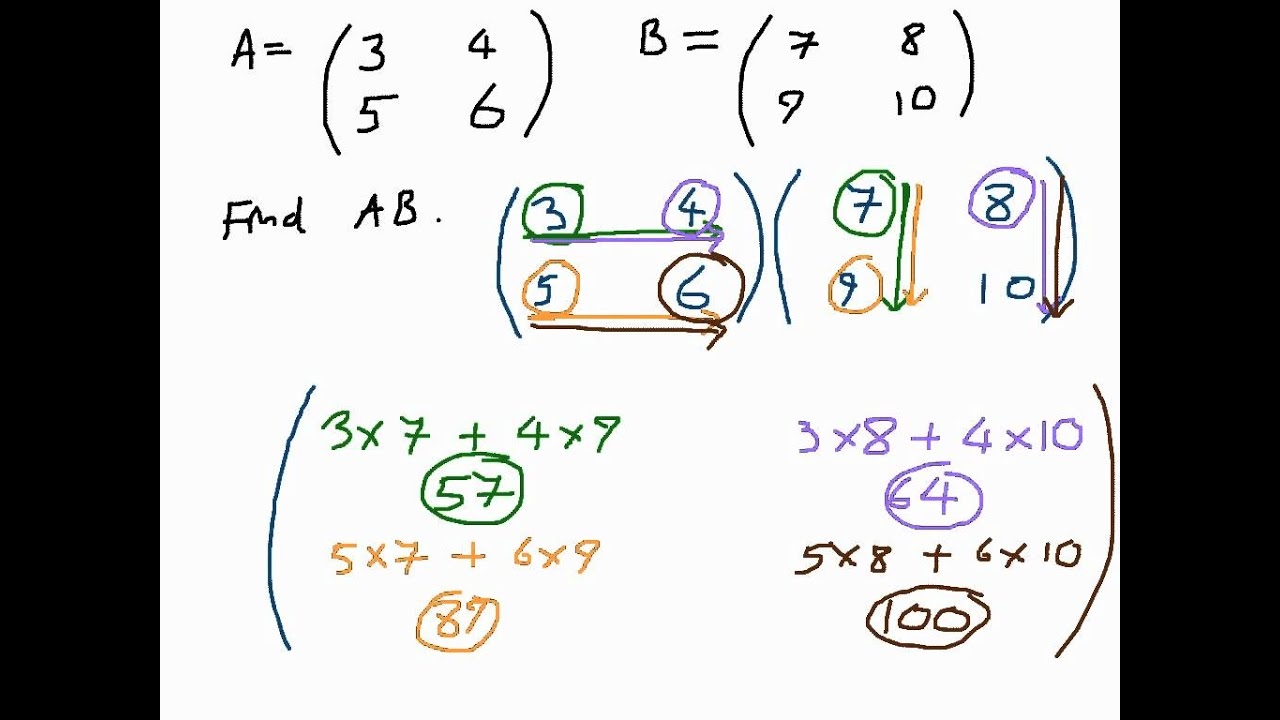
\includegraphics[width=0.8\textwidth]{media/matrix-mult.jpg}}
	\caption{Matrix multiplication as taught in American high school:
		``here's a recipe, trust me bro''. Image from \cite{img:matrixmult}.}
	\label{fig:matmult}
\end{figure}

\subsection{General discussion, back to Napkin levels of abstraction}
Let's go back to modern language,
where we work with finite-dimensional spaces over any field,
and any basis of the spaces (rather than a fixed basis like in the previous section).

Pick a finite-dimensional vector space $V$ with \emph{some} basis $e_1, \dots, e_m$
and a vector space $W$ with basis $w_1, \dots, w_n$.
Suppose I have a map $T \colon V \to W$ and I want to tell you what $T$ is.
It would be awfully inconsiderate of me to try and tell you what $T(v)$
is at every point $v$.
But we saw I only have to tell you what $T(e_1)$, \dots, $T(e_m)$ are,
because from there you can work out
$T(a_1 e_1 + \dots + a_m e_m)$ for yourself:
\[ T(a_1 e_1 + \dots + a_m e_m) = a_1 T(e_1) + \dots + a_m T(e_m). \]
Since the $e_i$ are a basis, that tells you all you need to know about $T$.
\begin{example}
	[Extending linear maps]
	Let $V = \left\{ ax^2+bx+c \mid a,b,c \in \RR \right\}$.
	Then $T(ax^2+bx+c) = aT(x^2) + bT(x) + cT(1)$.
\end{example}

Now I can even be more concrete.
I could tell you what $T(e_1)$ is, but seeing as I have a basis of $W$,
I can actually just tell you what $T(e_1)$ is in terms of this basis.
Specifically, there are unique $a_{11}, a_{21}, \dots, a_{n1} \in k$ such that
\[ T(e_1) = a_{11} w_1 + a_{21} w_2 + \dots + a_{n1} w_n. \]
So rather than telling you the value of $T(e_1)$ in some abstract space $W$,
I could just tell you what $a_{11}, a_{21}, \dots, a_{n1}$ were.
Then I'd repeat this for $T(e_2)$, $T(e_3)$, all the way up to $T(e_m)$,
and that would tell you everything you need to know about $T$.

That's where the matrix $T$ comes from!
It's a concise way of writing down all $mn$ numbers
I need to tell you.

To be explicit, the matrix for $T$ is defined as the array
\begin{align*}
	T &= \underbrace{%
	\begin{bmatrix}
		\mid & \mid & & \mid \\
		T(e_1) & T(e_2) & \dots & T(e_{m}) \\
		\mid & \mid & & \mid \\
	\end{bmatrix}
	}_{\text{$m$ columns}} \Bigg\} \text{$n$ rows} \\
	&=
	\begin{bmatrix}
		a_{11} & a_{12} & \dots & a_{1m} \\
		a_{21} & a_{22} & \dots & a_{2m} \\
		\vdots & \vdots & \ddots & \vdots \\
		a_{n1} & a_{n2} & \dots & a_{nm}
	\end{bmatrix}.
\end{align*}
To drive this point home,
\begin{moral}
	A matrix is the laziest possible way to specify
	a linear map from $V$ to $W$.
\end{moral}

\begin{example}
	[An example of a matrix]
	Here is a concrete example in terms of a basis.
	Let $V = \RR^3$ with basis $e_1$, $e_2$, $e_3$
	and let $W = \RR^2$ with basis $w_1$, $w_2$.
	If I have $T \colon V \to W$
	then uniquely determined by three values, for example:
	\begin{align*}
		T(e_1) &= 4w_1 + 7w_2 \\
		T(e_2) &= 2w_1 + 3w_2 \\
		T(e_3) &= w_1
	\end{align*}
	The columns then correspond to $T(e_1)$, $T(e_2)$, $T(e_3)$:
	\[
		T =
		\begin{bmatrix}
			4 & 2 & 1 \\
			7 & 3 & 0
		\end{bmatrix}
	\]
\end{example}

\begin{example}
	[An example of a matrix after choosing a basis]
	We again let $V = \left\{ ax^2 + bx + c \right\}$
	be the vector space of polynomials of degree at most $2$.
	We fix the basis $1$, $x$, $x^2$ for it.

	Consider the ``evaluation at $3$'' map,
	a map $V \to \RR$.
	We pick $1$ as the basis element of the RHS;
	then we can write it as a $1 \times 3$ matrix
	\[ \begin{bmatrix}
			1 & 3 & 9
		\end{bmatrix} \]
	with the columns corresponding to $T(1)$, $T(x)$, $T(x^2)$.
\end{example}

From here you can actually work out for yourself
what it means to multiply two matrices.
Suppose we have picked a basis for three spaces $U$, $V$, $W$.
Given maps $T \colon U \to V$ and $S \colon V \to W$,
we can consider their composition $S \circ T$, i.e.
\[ U \taking{T} V \taking{S} W. \]
Matrix multiplication is defined exactly so that the matrix $ST$
is the same thing we get from interpreting the composed function $S \circ T$ as a matrix,
as we saw last section.

In particular, since function composition is associative,
it follows that matrix multiplication is as well.

This means you can define concepts like the determinant or the trace of a matrix
both in terms of an ``intrinsic'' map $T \colon V \to W$
and in terms of the entries of the matrix.
Since the map $T$ itself doesn't refer to any basis,
the abstract definition will imply that the numerical definition
doesn't depend on the choice of a basis.

\section{Subspaces and picking convenient bases}
\prototype{Any two linearly independent vectors in $\RR^3$.}
% A submodule is exactly what you think it is.
\begin{definition}
	Let $M$ be a left $R$-module.
	A \vocab{submodule} $N$ of $M$ is a module $N$
	such that every element of $N$ is also an element of $M$.
	If $M$ is a vector space then $N$ is called a \vocab{subspace}.
\end{definition}

\begin{example}[Kernels]
	The \vocab{kernel} of a map $T \colon V \to W$ (written $\ker T$) is
	the set of $v \in V$ such that $T(v) = 0_W$.
	It is a subspace of $V$, since it's closed under addition and scaling (why?).
\end{example}
\begin{example}[Spans]
	Let $V$ be a vector space and $v_1, \dots, v_m$ be any vectors of $V$.
	The \vocab{span} of these vectors is defined as the set
	\[ \left\{ a_1 v_1 + \dots + a_m v_m \mid a_1, \dots, a_m \in k \right\}. \]
	Note that it is a subspace of $V$ as well!
\end{example}
\begin{ques}
	Why is $0_V$ an element of each of the above examples?
	In general, why must any subspace contain $0_V$?
\end{ques}

Subspaces behave nicely with respect to bases.
\begin{theorem}[Basis completion]
	\label{thm:basis_completion}
	Let $V$ be an $n$-dimensional space, and $V'$ a subspace of $V$.
	Then
	\begin{enumerate}[(a)]
		\ii $V'$ is also finite-dimensional.
		\ii If $e_1, \dots, e_m$ is a basis of $V'$, then there exist
		$e_{m+1}, \dots, e_n$ in $V$ such that
		$e_1, \dots, e_n$ is a basis of $V$.
	\end{enumerate}
\end{theorem}
\begin{proof}
	Omitted, since it is intuitive and the proof is not that enlightening.
	(However, we will use this result repeatedly later on,
	so do take the time to internalize it now.)
\end{proof}

A very common use case is picking a convenient basis for a map $T$.
\begin{theorem}[Picking a basis for linear maps]
	\label{thm:linear_map_basis}
	Let $T \colon V \to W$ be a map of finite-dimensional vector spaces,
	with $n = \dim V$, $m = \dim W$.
	Then there exists a basis $v_1, \dots, v_n$ of $V$
	and a basis $w_1, \dots, w_m$ of $W$,
	as well as a nonnegative integer $k$, such that
	\[
		T(v_i) =
		\begin{cases}
			w_i & \text{if $i \le k$} \\
			0_W & \text{if $i > k$}.
		\end{cases}
	\]
	Moreover $\dim \ker T = n-k$ and $\dim T\im(V) = k$.
\end{theorem}
\begin{proof}[Sketch of Proof]
	You might like to try this one yourself before reading on:
	it's a repeated application of \Cref{thm:basis_completion}.

	Let $\ker T$ have dimension $n-k$.
	We can pick $v_{k+1}, \dots, v_{n}$ a basis of $\ker T$.
	Then extend it to a basis $v_1, \dots, v_n$ of $V$.
	The map $T$ is injective over the span of $v_1, \dots, v_k$
	(since only $0_V$ is in the kernel) so its images in $W$ are linearly independent.
	Setting $w_i = T(v_i)$ for each $i$,
	we get some linearly independent set in $W$.
	Then extend it again to a basis of $W$.
\end{proof}

This theorem is super important,
not only because of applications but also
because it will give you the right picture in your head
of how a linear map is supposed to look.
I'll even draw a cartoon of it to make sure you remember:

\begin{center}
\begin{asy}
	unitsize(0.7cm);
	real d = 3;

	filldraw(box( (-3*d/2,3.5), (-d/2,-4.5) ), opacity(0.1)+lightcyan, blue);
	filldraw(box( (d/2,3.5), (3*d/2,-5.5) ), opacity(0.1)+lightred, red);

	label(scale(1.5)*"$V$", (-d,4), blue);
	dot("$e_1$", (-d,3), dir(180), blue);
	dot("$e_2$", (-d,2), dir(180), blue);
	label("$\vdots$", (-d,1), blue);
	dot("$e_k$", (-d,0), dir(180), blue);
	dot("$e_{k+1}$", (-d,-1), dir(180), blue);
	dot("$e_{k+2}$", (-d,-2), dir(180), blue);
	label("$\vdots$", (-d,-3), dir(180), blue);
	dot("$e_n$", (-d,-4), dir(180), blue);

	label(scale(1.5)*"$W$", (d,4), red);
	dot("$f_1$", (d,3), dir(0), red);
	dot("$f_2$", (d,2), dir(0), red);
	label("$\vdots$", (d,1), red);
	dot("$f_k$", (d,0), dir(0), red);
	dot("$f_{k+1}$", (d,-1), dir(0), red);
	dot("$f_{k+2}$", (d,-2), dir(0), red);
	dot("$f_{k+3}$", (d,-3), dir(0), red);
	label("$\vdots$", (d,-4), dir(0), red);
	dot("$f_m$", (d,-5), dir(0), red);

	label("$T$", (0,3), dir(90));
	draw( (-d,3)--(d,3), EndArrow, Margin(3,3) );
	draw( (-d,2)--(d,2), EndArrow, Margin(3,3) );
	draw( (-d,0)--(d,0), EndArrow, Margin(3,3) );
	draw( (-d,-1)--(0,-1), EndArrow, Margin(3,3) );
	draw( (-d,-2)--(0,-2), EndArrow, Margin(3,3) );
	draw( (-d,-4)--(0,-4), EndArrow, Margin(3,3) );
	label("$0$", (0,-1));
	label("$0$", (0,-2));
	label("$0$", (0,-4));

	draw( (5.5,3)--(6,3)--(6,0)--(5.5,0));
	label("$\operatorname{im} T$", (6, 1.5), dir(0));
	draw( (-5.5,-1)--(-6,-1)--(-6,-4)--(-5.5,-4) );
	label("$\ker T$", (-6, -2.5), dir(180));
\end{asy}
\end{center}

In particular, for $T \colon V \to W$,
one can write $V = \ker T \oplus V'$,
so that $T$ annihilates its kernel while sending $V'$
to an isomorphic copy in $W$.

A corollary of this (which you should have expected anyways)
is the so called rank-nullity theorem,
which is the analog of the first isomorphism theorem.
\begin{theorem}
	[Rank-nullity theorem]
	\label{thm:rank_nullity}
	Let $V$ and $W$ be finite-dimensional vector spaces.
	If $T \colon V \to W$, then
	\[ \dim V = \dim \ker T + \dim \img T. \]
\end{theorem}
\begin{ques}
	Conclude the rank-nullity theorem from \Cref{thm:linear_map_basis}.
\end{ques}

\section{A cute application: Lagrange interpolation}
Here's a cute application\footnote{Source: Communicated to me
by Joe Harris at the first Harvard-MIT Undergraduate Math Symposium.}
of linear algebra to a theorem from high school.
\begin{theorem}
	[Lagrange interpolation]
	Let $x_1, \dots, x_{n+1}$ be distinct real numbers
	and $y_1, \dots, y_{n+1}$ any real numbers.
	Then there exists a \emph{unique}
	polynomial $P$ of degree at most $n$
	such that \[ P(x_i) = y_i \] for every $i$.
\end{theorem}
When $n = 1$ for example, this loosely
says there is a unique line joining two points.
\begin{proof}
	The idea is to consider the vector space $V$
	of polynomials with degree at most $n$,
	as well as the vector space $W = \RR^{n+1}$.
	\begin{ques}
		Check that $\dim V = n + 1 = \dim W$.
		This is easiest to do if you pick a basis for $V$,
		but you can then immediately forget about the basis
		once you finish this exercise.
	\end{ques}
	Then consider the linear map $T \colon V \to W$ given by
	\[ P \mapsto \left( P(x_1), \dots, P(x_{n+1}) \right). \]
	This is indeed a linear map because,
	well, $T(P+Q) = T(P)+T(Q)$ and $T(cP) = cT(P)$.
	It also happens to be injective: if $P \in \ker T$,
	then $P(x_1) = \dots = P(x_{n+1}) = 0$,
	but $\deg P \le n$ and so $P$ can only be the zero polynomial.

	So $T$ is an injective map between vector spaces of the same dimension.
	Thus it is actually a bijection, which is exactly what we wanted.
\end{proof}

\section{Pedagogical digression: Arrays of numbers are evil}
\label{sec:basis_evil}

(This whole section is Evan yapping about how to \emph{teach} linear algebra,
so it can be safely skipped.)

As I'll stress repeatedly, a matrix represents a
\emph{linear map between two vector spaces}.
Writing it in the form of an $m \times n$ matrix
is merely a very convenient way to see the map concretely.
But it obfuscates the fact that this map is,
well, a map, not an array of numbers.

If you took high school precalculus, you'll see everything done in terms of matrices.
To any typical high school student, a matrix is an array of numbers.
No one is sure what exactly these numbers represent,
but they're told how to magically multiply these arrays to get more arrays.
They're told that the matrix
\[ \begin{bmatrix}
		1 & 0 & \dots & 0 \\
		0 & 1 & \dots & 0 \\
		\vdots & \vdots & \ddots & \vdots \\
		0 & 0 & \dots & 1 \\
	\end{bmatrix} \]
is an ``identity matrix'', because when you multiply
by another matrix it doesn't change.
Then they're told that the determinant is some magical combination of these
numbers formed by this weird multiplication rule.
No one knows what this determinant does,
other than the fact that $\det(AB) = \det A \det B$,
and something about areas and row operations and Cramer's rule.

Then you go into linear algebra in college, and you do more magic
with these arrays of numbers.
You're told that two matrices $T_1$ and $T_2$ are similar if
\[ T_2 = ST_1S\inv \] for some invertible matrix $S$.
You're told that the trace of a matrix $\Tr T$ is the sum of the diagonal entries.
Somehow this doesn't change if you look at a similar matrix,
but you're not sure why.
Then you define the characteristic polynomial as
\[ p_T(X) = \det (XI - T). \]
Somehow this also doesn't change if you take a similar matrix,
but now you really don't know why.
And then you have the Cayley-Hamilton theorem in all its black magic:
$p_T(T)$ is the zero map.  Out of curiosity you Google the proof,
and you find some ad-hoc procedure which still leaves you
with no idea why it's true.

This is terrible. What's so special about $T_2 = ST_1S\inv$?
Only if you know that the matrices are linear maps does this make sense:
$T_2$ is just $T_1$ rewritten with a different choice of basis.

I really want to push the opposite view.
Linear algebra is the study of \emph{linear maps},
but it is taught as the study of \emph{arrays of numbers},
and no one knows what these numbers mean.
And for a good reason: the numbers are meaningless.
They are a highly convenient way of encoding the matrix,
but they are not the main objects of study,
any more than the dates of events are the main objects of study in history.

The other huge downside is that people get the impression
that the only (real) vector space in existence is $\RR^{\oplus n}$.
As explained in \Cref{rem:vector_spaces_have_essence},
while you \emph{can} work this way if you're a soulless robot,
it's very unnatural for humans to do so.

When I took Math 55a as a freshman at Harvard,
I got the exact opposite treatment:
we did all of linear algebra without writing down a single matrix.
During all this time I was quite confused.
What's wrong with a basis?
I didn't appreciate until later that this approach was the
morally correct way to treat the subject: it made it clear what was happening.

Throughout the Napkin, I've tried to strike a balance between these
two approaches, using matrices when appropriate to illustrate
the maps and to simplify proofs, but ultimately writing
theorems and definitions in their \emph{morally correct} form.
I hope that this has both the advantage of giving the ``right'' definitions
while being concrete enough to be digested.
But I would like to say for the record that,
if I had to pick between the high school approach and the 55a approach,
I would pick 55a in a heartbeat.

\section{A word on general modules}
\prototype{$\ZZ[\sqrt2]$ is a $\ZZ$-module of rank two.}
I focused mostly on vector spaces (aka modules over a field) in this chapter
for simplicity, so I want to make a few remarks about
modules over a general commutative ring $R$ before concluding.

Firstly, recall that for general modules,
we say ``generating set'' instead of ``spanning set''.
Shrug.

The main issue with rings is that our key theorem \Cref{thm:vector_best}
fails in spectacular ways.
For example, consider $\ZZ$ as a $\ZZ$-module over itself.
Then $\{2\}$ is linearly independent, but it cannot be extended to a basis.
Similarly, $\{2,3\}$ is spanning, but one cannot cut it down to a basis.
You can see why defining dimension is going to be difficult.

Nonetheless, there are still analogs of some of the definitions above.
\begin{definition}
	An $R$-module $M$ is called \vocab{finitely generated} if it has a finite generating set.
\end{definition}
\begin{definition}
	An $R$-module $M$ is called \vocab{free} if it has a basis.
	As said before, the analogue of the dimension theorem holds,
	and we use the word \vocab{rank} to denote the size of the basis.
	As before, there's an isomorphism $M \cong R^{\oplus n}$ where $n$ is the rank.
\end{definition}
\begin{example}[An example of a $\ZZ$-module]
	The $\ZZ$-module
	\[ \ZZ[\sqrt2] = \left\{ a + b\sqrt 2 \mid a,b \in \ZZ \right\} \]
	has a basis $\{1, \sqrt 2\}$, so we say it is
	a free $\ZZ$-module of rank $2$.
\end{example}

\begin{abuse}
	[Notation for groups]
	Recall that an abelian group
	can be viewed a $\ZZ$-module (and in fact vice-versa!),
	so we can (and will) apply these words to abelian groups.
	We'll use the notation $G \oplus H$ for two abelian groups $G$ and $H$
	for their Cartesian product, emphasizing the fact that $G$ and $H$ are abelian.
	This will happen when we study algebraic number theory and homology groups.
\end{abuse}

\section{\problemhead}
General hint:
\Cref{thm:linear_map_basis} will be your best friend
for many of these problems.

\begin{dproblem}
	Let $V$ and $W$ be finite-dimensional vector spaces
	with nonzero dimension, and consider linear maps $T \colon V \to W$.
	Complete the following table by writing
	``sometimes'', ``always'', or ``never'' for each entry.
	\begin{center}
	\begin{tabular}[h]{c|ccc}
		& $T$ injective & $T$ surjective & $T$ isomorphism \\ \hline
		If $\dim V > \dim W$\dots \\
		If $\dim V = \dim W$\dots \\
		If $\dim V < \dim W$\dots \\
	\end{tabular}
	\end{center}
	\begin{hint}
		Use the rank-nullity theorem.
		Also consider the zero map.
	\end{hint}
	\begin{sol}
		\begin{center}
		\begin{tabular}[h]{c|ccc}
		& $T$ injective & $T$ surjective & $T$ isomorphism \\ \hline
		If $\dim V > \dim W$\dots & never & sometimes & never\\
		If $\dim V = \dim W$\dots & sometimes & sometimes & sometimes \\
		If $\dim V < \dim W$\dots & sometimes & never & never \\
		\end{tabular}
		\end{center}
		Each ``never'' is by the rank-nullity theorem.
		Each counterexample is obtained by the zero map
		sending every element of $V$ to zero;
		this map is certainly neither injective or surjective.
	\end{sol}
\end{dproblem}

\begin{dproblem}
	[Equal dimension vector spaces are usually isomorphisms]
	\label{prob:equal_dimension}
	Let $V$ and $W$ be finite-dimensional vector
	spaces with $\dim V = \dim W$.
	Prove that for a map $T \colon V \to W$,
	the following are equivalent:
	\begin{itemize}
		\ii $T$ is injective,
		\ii $T$ is surjective,
		\ii $T$ is bijective.
	\end{itemize}
	\begin{sol}
		It essentially follows by \Cref{thm:linear_map_basis}.
	\end{sol}
\end{dproblem}

\begin{problem}
	Let's say a \emph{magic square} is a $3 \times 3$ matrix of real numbers
	where the sum of all diagonals, columns, and rows is equal, such as
	$\left[ \begin{smallmatrix}
		8 & 1 & 6 \\
		3 & 5 & 7 \\
		4 & 9 & 2
	\end{smallmatrix} \right]$.
	Find the dimension of the set of magic squares, as a real vector space under addition.
\end{problem}

\begin{problem}
	[Multiplication by $\sqrt5$]
	Let $V = \QQ[\sqrt5] = \left\{ a + b \sqrt 5 \right\}$
	be a two-dimensional $\QQ$-vector space,
	and fix the basis $\{1, \sqrt 5\}$ for it.
	Write down the $2 \times 2$ matrix with rational coefficients
	that corresponds to multiplication by $\sqrt 5$.
	\begin{hint}
		$a + b \sqrt 5 \mapsto \sqrt 5 a + 5b$.
	\end{hint}
	\begin{sol}
		Since $1 \mapsto \sqrt5$ and $\sqrt5 \mapsto 5$,
		the matrix is
		$\begin{bmatrix}
			0 & 5 \\
			1 & 0
		\end{bmatrix}$.
	\end{sol}
\end{problem}

\begin{problem}
	[Multivariable Lagrange interpolation]
	Let $S \subset {\mathbb Z}^2$ be a set of $n$ lattice points.
	Prove that there exists a nonzero two-variable polynomial $p$
	with real coefficients, of degree at most $\sqrt{2n}$,
	such that $p(x,y) = 0$ for every $(x,y) \in S$.
\end{problem}

\begin{problem}
	[Putnam 2003]
	Do there exist polynomials $a(x)$, $b(x)$, $c(y)$, $d(y)$ such that
	\[ 1 + xy + (xy)^2 = a(x)c(y) + b(x)d(y) \]
	holds identically?
	\begin{hint}
		Plug in $y = -1, 0, 1$. Use dimensions of $\RR[x]$.
	\end{hint}
\end{problem}

\begin{problem}[TSTST 2014]
	\gim
	Let $P(x)$ and $Q(x)$ be arbitrary polynomials with real coefficients,
	and let $d$ be the degree of $P(x)$.
	Assume that $P(x)$ is not the zero polynomial.
	Prove that there exist polynomials $A(x)$ and $B(x)$ such that
	\begin{enumerate}[(i)]
		\ii Both $A$ and $B$ have degree at most $d/2$,
		\ii At most one of $A$ and $B$ is the zero polynomial,
		\ii $P$ divides $A+Q \cdot B$.
	\end{enumerate}
	\begin{hint}
		Interpret as $V \oplus V \to W$ for suitable $V$, $W$.
	\end{hint}
	\begin{sol}
		Let $V$ be the space of real polynomials with degree at most $d/2$
		(which has dimension $1 + \left\lfloor d/2 \right\rfloor$),
		and $W$ be the space of real polynomials modulo $P$ (which has dimension $d$).
		Then $\dim (V \oplus V) > \dim W$.
		So the linear map $V \oplus V \to W$ by $(A,B) \mapsto A + Q \cdot B$
		has a kernel of positive dimension
		(by rank-nullity, for example).
	\end{sol}
\end{problem}

\begin{sproblem}
	[Idempotents are projection maps]
	\label{prob:idempotent}
	Let $P \colon V \to V$ be a linear map,
	where $V$ is a vector space
	(not necessarily finite-dimensional).
	Suppose $P$ is \vocab{idempotent},
	meaning $P(P(v)) = P(v)$ for each $v \in V$,
	or equivalently $P$ is the identity on its image.
	Prove that \[ V = \ker P \oplus \img P. \]
	Thus we can think of $P$ as \emph{projection}
	onto the subspace $\img P$.
\end{sproblem}

\begin{sproblem}
	\label{prob:endomorphism_eventual_lemma}
	\gim
	Let $V$ be a finite dimensional vector space.
	Let $T \colon V \to V$ be a linear map,
	and let $T^n \colon V \to V$ denote $T$ applied $n$ times.
	Prove that there exists an integer $N$ such that
	\[ V = \ker T^N \oplus \img T^N. \]
	\begin{hint}
		Use the fact that the infinite chain of subspaces
		\[ \ker T \subseteq \ker T^2 \subseteq \ker T^3 \subseteq \dots \]
		and the similar chain for $\img T$ must eventually stabilize
		(for dimension reasons).
	\end{hint}
	\begin{sol}
		Consider
		\[
			\{0\} \subsetneq \ker S \subseteq \ker S^2 \subseteq \ker S^3 \subseteq \dots
			\text{  and  }
			V \supsetneq \img S \supseteq \img S^2 \supseteq \img S^3 \supseteq \dots.
		\]
		For dimension reasons, these subspaces must eventually stabilize:
		for some large integer $N$,
		$\ker T^N = \ker T^{N+1} = \dots$
		and $\img T^N = \img T^{N+1} = \img T^{N+2} = \dots$.
		When this happens, $\ker T^N \bigcap \img T^N = \{0\}$,
		since $T^N$ is an automorphism of $\img T^N$.
		On the other hand, by Rank-Nullity we also have
		$\dim \ker T^N + \dim \img T^n = \dim V$.
		Thus for dimension reasons, $V = \ker T^N \oplus \img T^N$.
	\end{sol}
\end{sproblem}

%Now consider the sequences
